\documentclass[journal,12pt,onecolumn]{IEEEtran}
\usepackage{cite}
\usepackage{graphicx}
\usepackage{amsmath,amssymb,amsfonts,amsthm}
\usepackage{algorithmic}
\usepackage{graphicx}
\usepackage{textcomp}
\usepackage{xcolor}
\usepackage{txfonts}
\usepackage{listings}
\usepackage{enumitem}
\usepackage{mathtools}
\usepackage{gensymb}
\usepackage{comment}
\usepackage[breaklinks=true]{hyperref}
\usepackage{tkz-euclide} 
\usepackage{listings}
\usepackage{gvv}                                        
%\def\inputGnumericTable{}                                 
\usepackage[latin1]{inputenc} 
\usetikzlibrary{arrows.meta, positioning}
\usepackage{xparse}
\usepackage{color}                                            
\usepackage{array}                                            
\usepackage{longtable}                                       
\usepackage{calc}                                             
\usepackage{multirow}
\usepackage{multicol}
\usepackage{hhline}                                           
\usepackage{ifthen}                                           
\usepackage{lscape}
\usepackage{tabularx}
\usepackage{array}
\usepackage{float}
\newtheorem{theorem}{Theorem}[section]
\newtheorem{problem}{Problem}
\newtheorem{proposition}{Proposition}[section]
\newtheorem{lemma}{Lemma}[section]
\newtheorem{corollary}[theorem]{Corollary}
\newtheorem{example}{Example}[section]
\newtheorem{definition}[problem]{Definition}
\newcommand{\BEQA}{\begin{eqnarray}}
\newcommand{\EEQA}{\end{eqnarray}}
\usepackage{float}
%\newcommand{\define}{\stackrel{\triangle}{=}}
\theoremstyle{remark}
\usepackage{circuitikz}
\usepackage{tikz}
\title{EC: ELECTRONICS AND COMMUNICATION ENGINEERING - 2013}
\author{EE25BTECH11037 - Divyansh}


\begin{document}
\maketitle

\begin{enumerate}

\item A bulb in a staircase has two switches, one switch being at the ground floor and the other one at the first floor. The bulb can be turned ON and also can be turned OFF by any one of the switches irrespective of the state of the other switch. The logic of switching of the bulb resembles
\begin{multicols}{4}
\begin{enumerate}
    \item an AND gate
    \item an OR gate
    \item an XOR gate
    \item a NAND gate
\end{enumerate}
\end{multicols}
\hfill \brak{\text{GATE EC 2013}}

\item Consider a vector field $\vec{A}(\vec{r})$. The closed loop line integral $\oint \vec{A} \cdot d\vec{l}$ can be expressed as
\begin{enumerate}
    \item $\iint_{\text{closed surface}} \brak{\nabla \times \vec{A}} \cdot d\vec{s}$
    \item $\iiint_{\text{closed volume}} \brak{\nabla \cdot \vec{A}} \, dv$
    \item $\iiint_{\text{open volume}} \brak{\nabla \cdot \vec{A}} \, dv$
    \item $\iint_{\text{open surface}} \brak{\nabla \times \vec{A}} \cdot d\vec{s}$
\end{enumerate}
\hfill \brak{\text{GATE EC 2013}}

\item Two systems with impulse responses $h_1\brak{t}$ and $h_2\brak{t}$ are connected in cascade. Then the overall impulse response of the cascaded system is given by
\begin{enumerate}
    \item product of $h_1\brak{t}$ and $h_2\brak{t}$
    \item sum of $h_1\brak{t}$ and $h_2\brak{t}$
    \item convolution of $h_1\brak{t}$ and $h_2\brak{t}$
    \item subtraction of $h_2\brak{t}$ from $h_1\brak{t}$
\end{enumerate}
\hfill \brak{\text{GATE EC 2013}}

\item In a forward biased pn junction diode, the sequence of events that best describes the mechanism of current flow is
\begin{enumerate}
    \item injection, and subsequent diffusion and recombination of minority carriers
    \item injection, and subsequent drift and generation of minority carriers
    \item extraction, and subsequent diffusion and generation of minority carriers
    \item extraction, and subsequent drift and recombination of minority carriers
\end{enumerate}
\hfill \brak{\text{GATE EC 2013}}

\item In IC technology, dry oxidation \brak{\text{using dry oxygen}} as compared to wet oxidation \text{\brak{using steam or water vapor}} produces
\begin{enumerate}
    \item superior quality oxide with a higher growth rate
    \item inferior quality oxide with a higher growth rate
    \item inferior quality oxide with a lower growth rate
    \item superior quality oxide with a lower growth rate
\end{enumerate}
\hfill \brak{\text{GATE EC 2013}}

\item The maximum value of $\theta$ until which the approximation $\sin{\theta} \approx \theta$ holds within the $10\%$ error is 
\begin{multicols}{4}
\begin{enumerate}
    \item $10^{\circ}$
    \item $18^{\circ}$
    \item $50^{\circ}$
    \item $90^{\circ}$
\end{enumerate}
\end{multicols}
\hfill \brak{\text{GATE EC 2013}}

\item The divergence of the vector field $\vec{A}=x\hat{a}_{x}+y\hat{a}_{y}+z\hat{a}_{z}$ is
\begin{multicols}{4}
 \begin{enumerate}
        \item $0$
        \item $1/3$
        \item $1$
        \item $3$
  \end{enumerate}
\end{multicols}
\hfill \brak{\text{GATE EC 2013}}

\item The impulse response of a system is $h\brak{t}=t u\brak{t}$. For an input $u(t-1)$, the output is
\begin{multicols}{4}
    \begin{enumerate}
        \item $\frac{t^{2}}{2}u\brak{t}$
        \item $\frac{t\brak{t-1}}{2}u\brak{t-1}$
        \item $\frac{\brak{t-1}^{2}}{2}u\brak{t-1}$
        \item $\frac{t^{2}-1}{2}u\brak{t-1}$
    \end{enumerate}
\end{multicols}
\hfill \brak{\text{GATE EC 2013}}

\item The Bode plot of a transfer function $G\brak{s}$ is shown in the $\figref{fig:placeholder_1}$ below.
\begin{figure}[H]
    \centering
    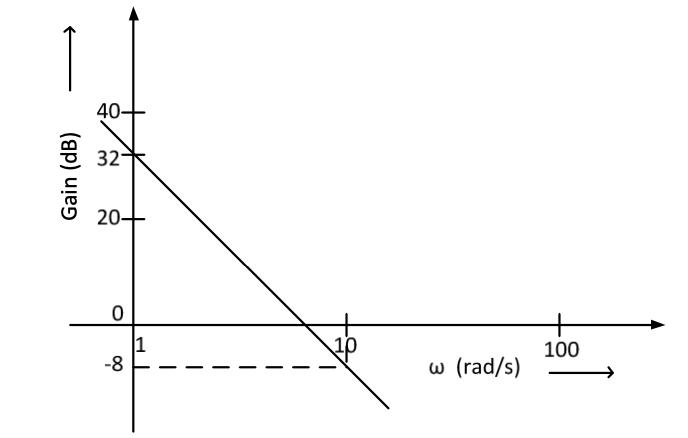
\includegraphics[width=0.5\columnwidth]{figs/fig_1.png}
    \caption{\centering for q-9}
    \label{fig:placeholder_1}
\end{figure}

The gain $\brak{20 \log |G\brak{s}|}$ is $32 dB$ and $-8 dB$ at $1 rad/s$ and $10 rad/s$ respectively. The phase is negative for all $\omega$. Then $G\brak{s}$ is
\begin{multicols}{4}
    \begin{enumerate}
        \item $\frac{39.8}{s}$
        \item $\frac{39.8}{s^2}$
        \item $\frac{32}{s}$
        \item $\frac{32}{s^2}$
    \end{enumerate}
\end{multicols}
\hfill \brak{\text{GATE EC 2013}}

\item In the circuit shown below in $\figref{fig:placeholder_2}$ what is the output voltage $\brak{V_{out}}$ if a silicon transistor $Q$ and an ideal op-amp are used?
\begin{figure}[H]
    \centering
    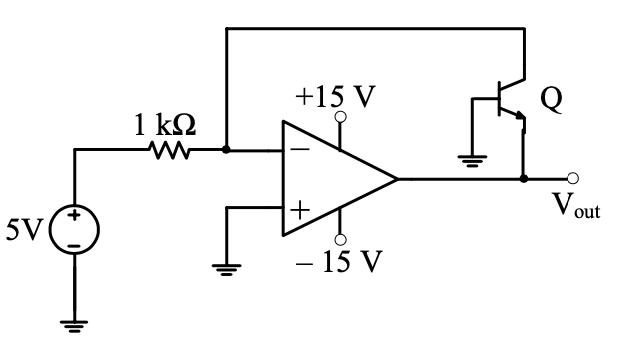
\includegraphics[width=0.5\columnwidth]{figs/fig_2.png}
    \caption{\centering for q-10}
    \label{fig:placeholder_2}
\end{figure}
\begin{multicols}{4}
    \begin{enumerate}
        \item $-15 V$
        \item $-0.7 V$
        \item $+0.7 V$
        \item $+15 V$
    \end{enumerate}
\end{multicols}
\hfill \brak{\text{GATE EC 2013}}

\item Consider a delta connection of resistors and its equivalent star connection as shown below in $\figref{fig:placeholder_3}$. If all elements of the delta connection are scaled by a factor $k$, $k> 0$, the elements of the corresponding star equivalent will be scaled by a factor of 
\begin{figure}[H]
    \centering
    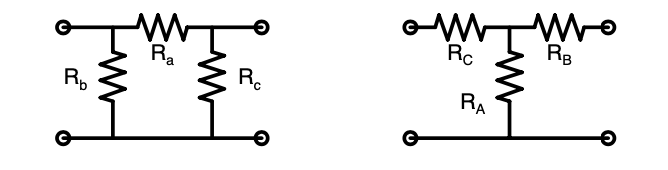
\includegraphics[width=0.5\columnwidth]{figs/fig_3.png}
    \caption{\centering for q-11}
    \label{fig:placeholder_3}
\end{figure}
\begin{multicols}{4}
    \begin{enumerate}
        \item $k^2$
        \item $k$
        \item $\frac{1}{k}$
        \item $\sqrt{k}$
    \end{enumerate}
\end{multicols}
\hfill \brak{\text{GATE EC 2013}}

\item For $8085$ microprocessor, the following program is executed.
\begin{verbatim}
    MVI A, 05H;
    MVI B, 05H;
PTR:ADD B;
    DCR B;
    JNZ PTR;
    ADI 03H;
    HLT;
\end{verbatim}
At the end of program, accumulator contains
\begin{multicols}{4}
    \begin{enumerate}
        \item $17H$
        \item $20H$
        \item $23H$
        \item $05H$
    \end{enumerate}
\end{multicols}
\hfill \brak{\text{GATE EC 2013}}

\item The bit rate of a digital communication system is $R\ kbits/s$. The modulation used is $32-QAM$. The minimum bandwidth required for ISI free transmission is
\begin{multicols}{4}
    \begin{enumerate}
        \item $R/10 \ Hz$
        \item $R/10 \ kHz$
        \item $R/5 \ Hz$
        \item $R/5 \ kHz$
    \end{enumerate}
\end{multicols}
\hfill \brak{\text{GATE EC 2013}}

\item For a periodic signal $v\brak{t} = 30 \sin 100 t +10 \cos 300 t + 6 \sin \brak{500 t + \pi / 4}$ , the fundamental frequency in $rad/s$ is
\begin{multicols}{4}
    \begin{enumerate}
        \item $100$
        \item $300$
        \item $500$
        \item $1500$
    \end{enumerate}
\end{multicols}
\hfill \brak{\text{GATE EC 2013}}

\item In a voltage-voltage feedback as shown below in the $\figref{fig:placeholder_4}$, which one of the following statements is TRUE if the gain $k$ is increased?
\begin{figure}[H]
    \centering
    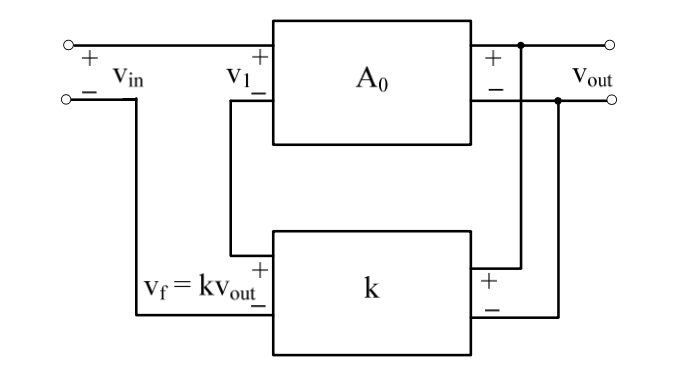
\includegraphics[width=0.5\columnwidth]{figs/fig_4.png}
    \caption{\centering for q-15}
    \label{fig:placeholder_9}
\end{figure}
\begin{enumerate}
\item  The input impedance increases and output impedance decreases.
\item  The input impedance increases and output impedance also increases. 
\item  The input impedance decreases and output impedance also decreases. 
\item  The input impedance decreases and output impedance increases.
\end{enumerate}
\hfill \brak{\text{GATE EC 2013}}

\item A band-limited signal with a maximum frequency of 5 kHz is to be sampled. According to the sampling theorem, the sampling frequency which is not valid is
\begin{multicols}{4}
\begin{enumerate}
\item $5 kHz$
\item $12 kHz$
\item $15 kHz$
\item $20 kHz$
\end{enumerate}
\end{multicols}
\hfill \brak{\text{GATE EC 2013}}

\item In a MOSFET operating in the saturation region, the channel length modulation effect causes
\begin{enumerate}
\item an increase in the gate-source capacitance
\item a decrease in the transconductance
\item a decrease in the unity-gain cutoff frequency
\item a decrease in the output resistance
\end{enumerate}
\hfill \brak{\text{GATE EC 2013}}

\item Which one of the following statements is NOT TRUE for a continuous time causal and stable LTI system?
\begin{enumerate}
\item All the poles of the system must lie on the left side of the $j\omega$ axis
\item Zeros of the system can lie anywhere in the $s-plane$
\item All the poles must lie within $|s| = 1$
\item All the roots of the characteristic equation must be located on the left side of the $j\omega$ axis
\end{enumerate}
\hfill \brak{\text{GATE EC 2013}}

\item The minimum eigenvalue of the following matrix is  
\begin{align*}
    \myvec{ 3 & 5 & 2 \\ 5 & 12 & 7 \\ 2 & 7 & 5 }
\end{align*}

\begin{multicols}{4}
  \begin{enumerate}
\item 0
\item 1
\item 2
\item 3
\end{enumerate}
\end{multicols}
\hfill \brak{\text{GATE EC 2013}}

\item A polynomial $f\brak{x} = a_4x^4 + a_3x^3 + a_2x^2 + ax - a_0$ with all coefficients positive has
\begin{multicols}{2}
\begin{enumerate}
\item no real roots
\item no negative real root
\item odd number of real roots
\item at least one positive and one negative real root
\end{enumerate}
\end{multicols}
\hfill \brak{\text{GATE EC 2013}}

\item Assuming zero initial condition, the response $y\brak{t}$ of the system given below in the $\figref{fig:placeholder_5}$ to a unit step input $u\brak{t}$ is  
\begin{figure}[H]
    \centering
    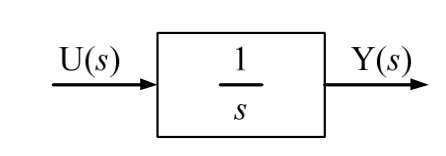
\includegraphics[width=0.5\columnwidth]{figs/fig_5.png}
    \caption{\centering for q-21}
    \label{fig:placeholder_5}
\end{figure}
\begin{multicols}{4}
\begin{enumerate}
\item $u\brak{t}$
\item $t u\brak{t}$
\item $\frac{t^2}{2} u\brak{t}$
\item $e^{-t} u\brak{t}$
\end{enumerate}
\end{multicols}
\hfill \brak{\text{GATE EC 2013}}

\item The transfer function $\frac{V_2\brak{s}}{V_1\brak{s}}$ of the circuit shown below in $\figref{fig:placeholder_6}$ is  
\begin{figure}[H]
    \centering
    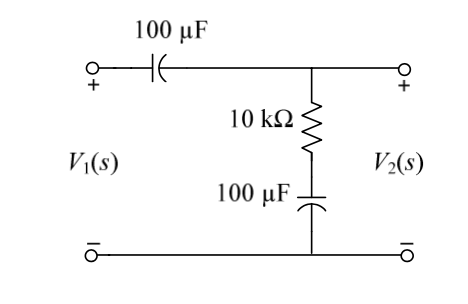
\includegraphics[width=0.5\columnwidth]{figs/fig_6.png}
    \caption{\centering for q-22}
    \label{fig:placeholder_6}
\end{figure}

\begin{multicols}{2}
\begin{enumerate}
\item $\frac{0.5s + 1}{s + 1}$
\item $\frac{3s + 6}{s + 2}$
\item $\frac{s + 2}{s + 1}$
\item $\frac{s + 2}{s + 2}$
\end{enumerate}
\end{multicols}
\hfill \brak{\text{GATE EC 2013}}

\item A source $v\brak{t} = V \cos\brak{100\pi t}$ has an internal impedance of $(4 + j3)\,\ohm$. If a purely resistive load connected to this source has to extract the maximum power out of the source, its value in $\ohm$ should be
\begin{multicols}{4}
\begin{enumerate}
\item 3
\item 4
\item 5
\item 7
\end{enumerate}
\end{multicols}
\hfill \brak{\text{GATE EC 2013}}

\item The return loss of a device is found to be 20 dB. The voltage standing wave ratio \brak{VSWR} and magnitude of reflection coefficient are respectively
\begin{multicols}{4}
\begin{enumerate}
    \item $1.22 \ and \ 0.1$
    \item $0.81 \ and \  0.1$
    \item $-1.22 \ and  \ 0.1$
    \item $2.44 \ and \ 0.2$
\end{enumerate}
\end{multicols}
\hfill \brak{\text{GATE EC 2013}}

\item Let $g\brak{t} = e^{-\pi t^2}$, and $h\brak{t}$ is a filter matched to $g\brak{t}$. If $g\brak{t}$ is applied as input to $h\brak{t}$, then the Fourier transform of the output is

\begin{multicols}{4}
\begin{enumerate}
\item $e^{-\pi f^2}$
\item $e^{-\pi f^2/2}$
\item $e^{-\pi |f|}$
\item $e^{-2\pi f^2}$
\end{enumerate}
\end{multicols}
\hfill \brak{\text{GATE EC 2013}}

\item Let $U$ and $V$ be two independent zero mean Gaussian random variables of variances $1$ and $\frac{4}{9}$ respectively. The probability $P\brak{3V \geq 2U}$ is

\begin{multicols}{4}
\begin{enumerate}
\item $\frac{4}{9}$
\item $\frac{1}{2}$
\item $\frac{2}{3}$
\item $\frac{5}{9}$
\end{enumerate}
\end{multicols}
\hfill \brak{\text{GATE EC 2013}}


\item Let $A$ be an $m \times n$ matrix and $B$ an $n \times m$ matrix. It is given that $\det\brak{I_m + AB} = \det\brak{I_m + AB}$. Using this property, the determinant of the matrix
$\myvec{2 & 1 & 1 & 1 \\
1 & 2 & 1 & 1 \\
1 & 1 & 2 & 1 \\
1 & 1 & 1 & 2}$
is
\begin{multicols}{4}
\begin{enumerate}
\item 2
\item 5
\item 8
\item 16
\end{enumerate}
\end{multicols}
\hfill \brak{\text{GATE EC 2013}}

\item In the circuit shown below in $\figref{fig:placeholder_7}$, if the source voltage $V_s = 100\angle 253.13^\circ$ V, then the Thevenin's equivalent voltage in Volts as seen by the load resistance $R_L$ is
\begin{figure}[H]
    \centering
    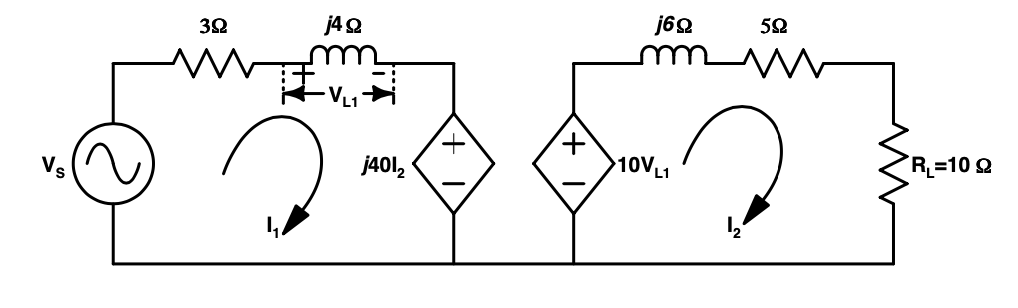
\includegraphics[width=0.5\columnwidth]{figs/fig_7.png}
    \caption{\centering for q-28}
    \label{fig:placeholder_7}
\end{figure}
\begin{multicols}{4}
\begin{enumerate}
\item $100\angle 90^\circ$
\item $800\angle 0^\circ$
\item $800\angle 90^\circ$
\item $100\angle 60^\circ$
\end{enumerate}
\end{multicols}
\hfill \brak{\text{GATE EC 2013}}

\item The open-loop transfer function of a DC motor is given as.$\frac{\theta(s)}{V_a(s)} = \frac{10}{1 + 10s}$. When connected in feedback, the approximate value of $K_a$ that will reduce the time constant of the closed-loop system by one hundred times compared to the open-loop system is
\begin{figure}[H]
    \centering
    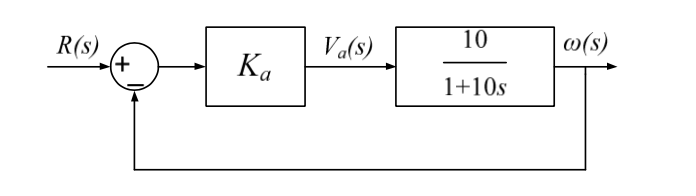
\includegraphics[width=0.5\columnwidth]{figs/fig_8.png}
    \caption{for q-29}
    \label{fig:placeholder_8}
\end{figure}
\begin{multicols}{4}
\begin{enumerate}
\item 1
\item 5
\item 10
\item 100
\end{enumerate}
\end{multicols}
\hfill \brak{\text{GATE EC 2013}}

\item In the circuit shown below in $\figref{fig:placeholder_9}$, the knee current of the ideal Zener diode is $10 mA$. To maintain $5 V$ across $R_L$, the minimum value of $R_L$ in $\ohm$ and the minimum power rating of the Zener diode in $mW$, respectively, are
\begin{figure}[H]
    \centering
    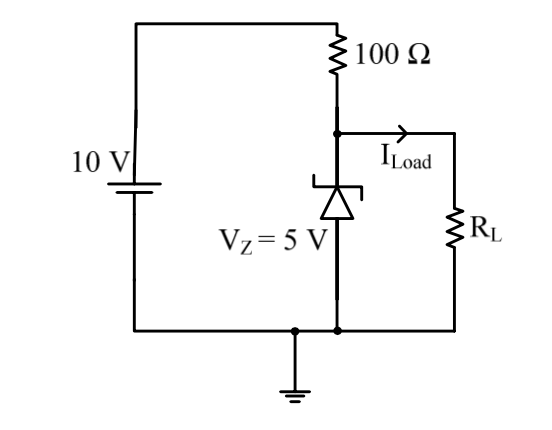
\includegraphics[width=0.5\columnwidth]{figs/fig_9.png}
    \caption{for q-30}
    \label{fig:placeholder_9}
\end{figure}
\begin{enumerate}
\item 125 and 125
\item 125 and 250
\item 250 and 125
\item 250 and 250
\end{enumerate}
\hfill \brak{\text{GATE EC 2013}}

\item The following arrangement consists of an ideal transformer and an attenuator which attenuates by a factor of 0.8. An AC voltage $V_{WX1} = 100 V$  is applied across $WX$ to get an open circuit voltage $V_{YZ1}$ across $YZ$. Next, an AC voltage $V_{YZ2} = 100$ V is applied across $YZ$ to get an open circuit voltage $V_{WX2}$ across $WX$. Then, $V_{YZ1}/V_{WX1}$ and $V_{WX2}/V_{YZ2}$ are respectively
\begin{figure}[H]
    \centering
    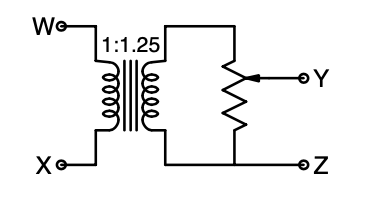
\includegraphics[width=0.5\columnwidth]{figs/fig_10.png}
    \caption{for q-31}
    \label{fig:placeholder_10}
\end{figure}
\begin{multicols}{2}
\begin{enumerate}
\item 125/100 and 80/100
\item 100/100 and 80/100
\item 100/100 and 100/100
\item 80/100 and 80/100
\end{enumerate}
\end{multicols}
\hfill \brak{\text{GATE EC 2013}}

\item Two magnetically uncoupled inductive coils have $Q$ factors $q_1$ and $q_2$ at the chosen operating frequency. Their respective resistances are $R_1$ and $R_2$. When connected in series, their effective $Q$ factor at the same operating frequency is
\begin{multicols}{2}
\begin{enumerate}
\item $q_1 + q_2$
\item $\brak{\frac{1}{q_1}} + \brak{\frac{1}{q_2}}$
\item $\frac{\brak{q_1 R_1 + q_2 R_2}}{\brak{R_1 + R_2}}$
\item $\frac{\brak{q_1 R_2 + q_2 R_1}}{R_1 + R_2}$
\end{enumerate}
\end{multicols}
\hfill \brak{\text{GATE EC 2013}}

\item The impulse response of a continuous-time system is given by $h\brak{t} = \delta\brak{t - 1} + \delta\brak{t - 3}$. The value of the step response at $t = 2$ is
\begin{multicols}{4}
\begin{enumerate}
\item 0
\item 1
\item 2
\item 3
\end{enumerate}
\end{multicols}
\hfill \brak{\text{GATE EC 2013}}

\item The small-signal resistance (i.e., $dV_B/dI_D$) in k$\ohm$ offered by the n-channel MOSFET $M$ shown in the $\figref{fig:placeholder_11}$ below, at a bias point of $V_B = 2$ V is (device data for $M$: transconductance parameter $K_N = \mu_n C_{ox} \brak{W/L} = 40$ $\mu$A/V$^2$, threshold voltage $V_{TN} = 1$ V, neglect body effect and channel length modulation).
\begin{figure}[H]
    \centering
    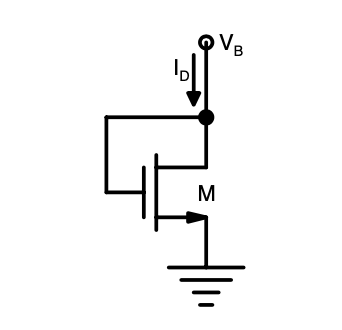
\includegraphics[width=0.5\columnwidth]{figs/fig_11.png}
    \caption{for q-34}
    \label{fig:placeholder_11}
\end{figure}
\begin{multicols}{4}
\begin{enumerate}
\item 12.5
\item 25
\item 50
\item 100
\end{enumerate}
\end{multicols}
\hfill \brak{\text{GATE EC 2013}}

\item The ac schematic of an NMOS common-source stage is shown below in $\figref{fig:placeholder_12}$, where part of the biasing circuits has been omitted for simplicity. For the n-channel MOSFET $M$, the transconductance $g_m = 1 \ mA/V$ , and body effect and channel length modulation effect are to be neglected. The lower cutoff frequency in Hz of the circuit is approximately
\begin{figure}[H]
    \centering
    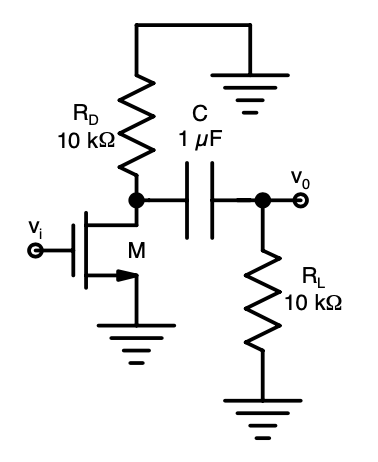
\includegraphics[width=0.5\columnwidth]{figs/fig_12.png}
    \caption{for q-35}
    \label{fig:placeholder_12}
\end{figure}
\begin{multicols}{4}
\begin{enumerate}
\item 8
\item 32
\item 50
\item 200
\end{enumerate}
\end{multicols}
\hfill \brak{\text{GATE EC 2013}}



\item A system is described by the differential equation
$\frac{d^2 y}{dt^2} + 5 \frac{dy}{dt} + 6y\brak{t} = x\brak{t}$
Let \brak{ x\brak{t} } be a rectangular pulse given by
$
x\brak{t} = \begin{cases}
10, & 0 < t < 2 \\
0, & \text{otherwise}
\end{cases}
$


Assuming \brak{ y\brak{0} = 0} and \brak{ \frac{dy}{dt} = 0 } at \brak{ t = 0 }, the Laplace transform of \brak{ y\brak{t} } is
\begin{multicols}{2}
\begin{enumerate}
\item \brak{ \frac{e^{-2s}}{s\brak{s+2}\brak{s+3}} }
\item \brak{ \frac{1 - e^{-2s}}{s\brak{s+2}\brak{s+3}} }
\item \brak{ \frac{e^{-2s}}{\brak{s+2}\brak{s+3}} }
\item \brak{ \frac{1 - e^{-2s}}{\brak{s+2}\brak{s+3}} }
\end{enumerate}
\end{multicols}
\hfill \brak{\text{GATE EC 2013}}

\item A system described by a linear, constant coefficient, ordinary, first order differential equation has an exact solution given by \brak{ y\brak{t} } for \brak{ t > 0 }, when the forcing function is \brak{ x\brak{t} } and the initial condition is \brak{ y\brak{0} }. If one wishes to modify the system so that the solution becomes \brak{ -2y\brak{t}}for \brak{ t > 0 }, we need to
\begin{enumerate}
\item change the initial condition to -y\brak{0} and the forcing function to 2x\brak{t}
\item change the initial condition to 2y\brak{0} and the forcing function to -x\brak{t}
\item change the initial condition to $j\sqrt{2}y\brak{0}$ and the forcing function to $j\sqrt{2} x\brak{t}$
\item change the initial condition to -2y\brak{0} and the forcing function to -2x\brak{t}
\end{enumerate}
\hfill \brak{\text{GATE EC 2013}}

\item Consider two identically distributed zero-mean random variables $U$ and $V$. Let the cumulative distribution functions of $U$ and $U$ be $F\brak{x}$  and $G\brak{x}$ respectively. Then, for all values of  $x$
\begin{multicols}{2}
\begin{enumerate}
\item  $F\brak{x} - G\brak{x} \leq 0 $
\item  $F\brak{x} - G\brak{x} \geq 0 $
\item  $\brak{F\brak{x} - G\brak{x}} \cdot x \leq 0 $
\item $ \brak{F\brak{x} - G\brak{x}} \cdot x \geq 0 $
\end{enumerate}
\end{multicols}
\hfill \brak{\text{GATE EC 2013}}

\item The DFT of a vector \myvec{a&&b&&c&&d} is the vector \myvec{A&&B&&Y&&\Theta}. Consider the product


$\myvec{p&&q&&r&&s} = \myvec{a&&b&&c&&d} \cdot
\myvec{
a & b & c & d \\
d & a & b & c \\
c & d & a & b \\
b & c & d & a}$


The DFT of the vector \myvec{p&&q&&r&&s} is a scaled version of
\begin{multicols}{2}
\begin{enumerate}
\item $\myvec{\alpha^2&&\beta^2&&\gamma^2&&\delta^2}$
\item $\myvec{\alpha+ \beta&&\beta+\delta &&\delta+\gamma&&\gamma + \alpha}$
\item $\myvec{\sqrt{\alpha}&&\sqrt{\beta}&&\sqrt{\gamma}&&\sqrt{\delta}}$
\item $\myvec{\alpha&&\beta&&\gamma&&\delta}$
\end{enumerate}
\end{multicols}
\hfill \brak{\text{GATE EC 2013}}

\item The signal flow graph for a system is given below in $\figref{fig:placeholder_13}$. The transfer function \brak{ \frac{Y\brak{s}}{U\brak{s}} } for this system is
\begin{figure}[H]
    \centering
    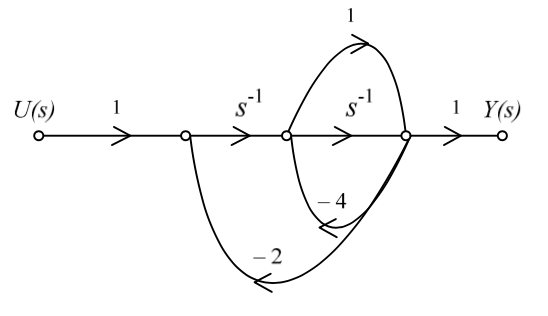
\includegraphics[width=0.5\columnwidth]{figs/fig_13.png}
    \caption{for q-40}
    \label{fig:placeholder_13}
\end{figure}

\begin{multicols}{2}

\begin{enumerate}
\item $\frac{1}{s^2 + 6s + 2}$
\item  $\frac{1}{5s^2 + 6s + 2}$ 
\item  $\frac{s + 1}{s^2 + 6s + 2}$
\item  $\frac{s + 1}{5s^2 + 6s + 2}$ 
\end{enumerate}
\end{multicols}
\hfill \brak{\text{GATE EC 2013}}

\item In the circuit shown below in $\figref{fig:placeholder_14}$ the op-amps are ideal. Then $V_{\text{out}}$ in Volts is
\begin{figure}[H]
    \centering
    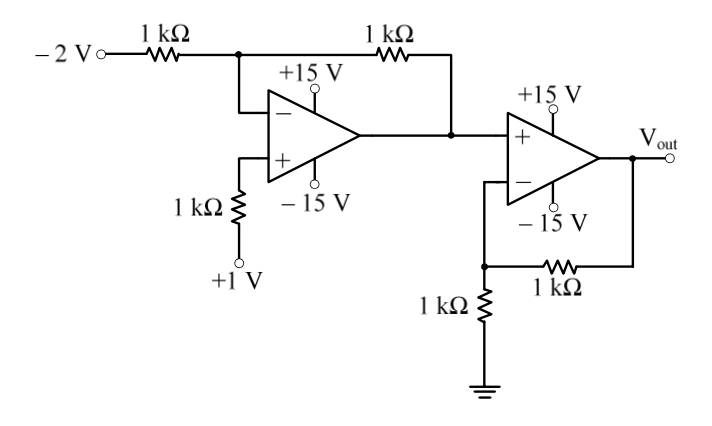
\includegraphics[width=0.5\columnwidth]{figs/fig_14.png}
    \caption{for q-41}
    \label{fig:placeholder_14}
\end{figure}
\begin{multicols}{4}
\begin{enumerate}
\item 4
\item 6
\item 8
\item 10
\end{enumerate}
\end{multicols}
\hfill \brak{\text{GATE EC 2013}}

\item In the circuit shown below in $\figref{fig:placeholder_15}$, $Q1$ has negligible collector-to-emitter saturation voltage and the diode drops negligible voltage across it under forward bias. If $V_{cc}$ is $+5 V$,$ X$ and $Y$ are digital signals with $0 V$ as logic $0$ and $V_{cc}$ as logic 1, then the Boolean expression for $Z$ is
\begin{figure}[H]
    \centering
    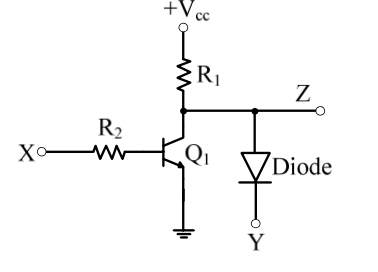
\includegraphics[width=0.5\columnwidth]{figs/fig_15.png}
    \caption{for q-42}
    \label{fig:placeholder_15}
\end{figure}
\begin{multicols}{4}
\begin{enumerate}
\item $XY$
\item $\overline{XY}$
\item $X + Y$
\item $\overline{X + Y}$
\end{enumerate}
\end{multicols}
\hfill \brak{\text{GATE EC 2013}}

\item A voltage $1000 \sin \omega t$ Volts is applied across $YZ$. Assuming ideal diodes, the voltage measured across $WX$ in Volts is
\begin{figure}[H]
    \centering
    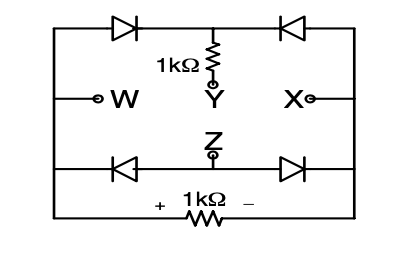
\includegraphics[width=0.5\columnwidth]{figs/fig_16.png}
    \caption{for q-43}
    \label{fig:placeholder_16}
\end{figure}
\begin{multicols}{2}
\begin{enumerate}
\item $\sin \omega t$
\item $\brak{\frac{\sin \omega t + |\sin \omega t|}{2}}$
\item $\brak{\frac{\sin \omega t - |\sin \omega t|}{2}}$
\item 0 for all $t$
\end{enumerate}
\end{multicols}
\hfill \brak{\text{GATE EC 2013}}

\item Three capacitors $C_1$, $C_2$ and $C_3$ whose values are $10$ $\mu$F, 5 $\mu$F, and 2 $\mu$F respectively, have breakdown voltages of $10 V$, $5 V$, and $2 V$ respectively. For the interconnection shown below, the maximum safe voltage in Volts that can be applied across the combination, and the corresponding total charge in $\mu$C stored in the effective capacitance across the terminals are respectively
\begin{figure}[H]
    \centering
    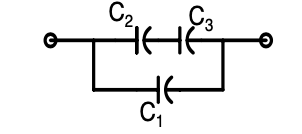
\includegraphics[width=0.5\columnwidth]{figs/fig_17.png}
    \caption{for q-44}
    \label{fig:placeholder_17}
\end{figure}
\begin{multicols}{2}
\begin{enumerate}
\item 2.8 and 36
\item 7 and 119
\item 2.8 and 32
\item 7 and 80
\end{enumerate}
\end{multicols}
\hfill \brak{\text{GATE EC 2013}}

\item There are four chips each of $1024 $ bytes connected to a $16-bit$ address bus as shown in the $\figref{fig:placeholder_18}$ below. RAMs 1, 2, 3 and 4 respectively are mapped to addresses
\begin{figure}[H]
    \centering
    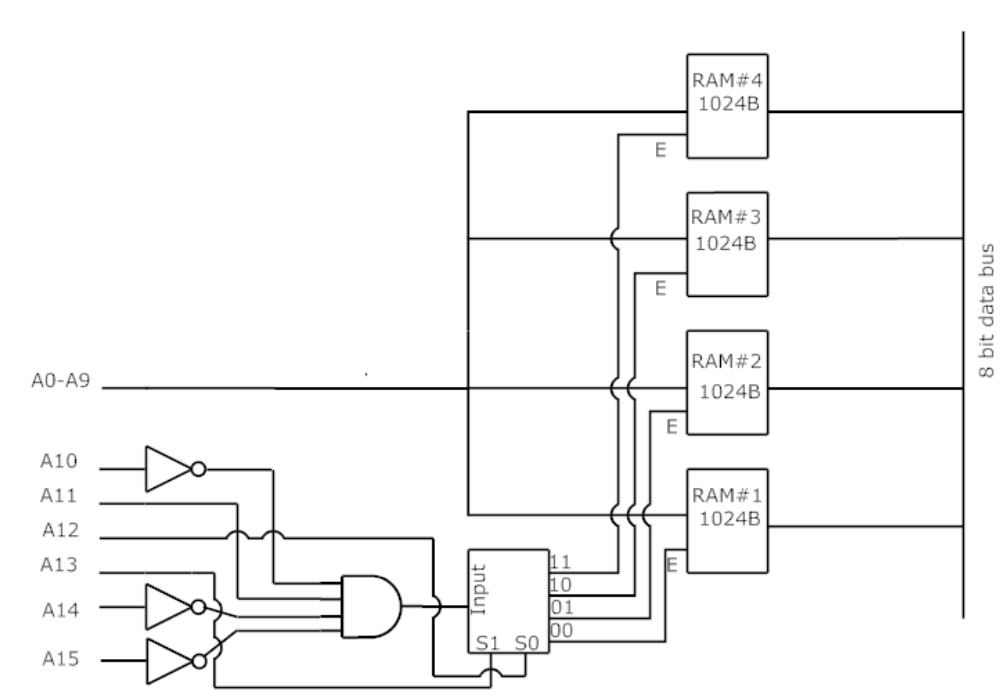
\includegraphics[width=0.5\columnwidth]{figs/fig_18.png}
    \caption{for q-45}
    \label{fig:placeholder_18}
\end{figure}

\begin{enumerate}
\item 0C00H–0FFFH, 1C00H–1FFFH, 2C00H–2FFFH, 3C00H–3FFFH
\item 1800H–1FFFH, 2800H–2FFFH, 3800H–3FFFH, 4800H–4FFFH
\item 0500H–08FFH, 1500H–18FFH, 3500H–38FFH, 5500H–58FFH
\item 0800H–0BFFH, 1800H–1BFFH, 2800H–2BFFH, 3800H–3BFFH
\end{enumerate}
\hfill \brak{\text{GATE EC 2013}}

\item In the circuit shown  below in $\figref{fig:placeholder_19}$, the silicon npn transistor $Q$ has a very high value of $\beta$. The required value of $R_2$ in $k \ohm$ to produce $I_C = 1$ mA is
\begin{figure}[H]
    \centering
    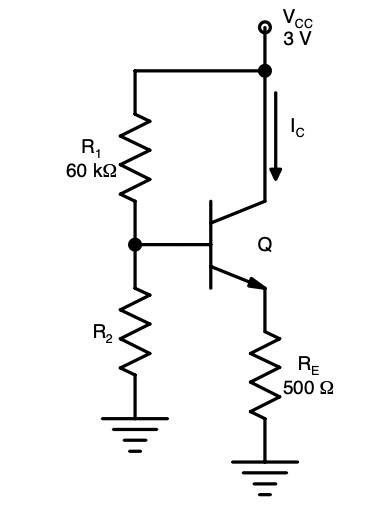
\includegraphics[width=0.5\columnwidth]{figs/fig_19.png}
    \caption{for q-46}
    \label{fig:placeholder_19}
\end{figure}
\begin{multicols}{4}
\begin{enumerate}
\item 20
\item 30
\item 40
\item 50
\end{enumerate}
\end{multicols}
\hfill \brak{\text{GATE EC 2013}}

\item Let $U$ and $V$ be two independent and identically distributed random variables such that $P\brak{U = +1} = P\brak{U = -1} = \frac{1}{2}$. The entropy $H\brak{U + V}$ in bits is

\begin{multicols}{4}
\begin{enumerate}
\item $\frac{3}{4}$
\item 1
\item $\frac{3}{2}$
\item $\log_2 3$
\end{enumerate}
\end{multicols}
\hfill \brak{\text{GATE EC 2013}}

Common data for q-48 and q-49

 Bits 1 and 0 are transmitted with equal probability. At the receiver, the pdf of the respective received signals for both bits are as shown below in $\figref{fig:placeholder_20}$.
 \begin{figure}[H]
    \centering
    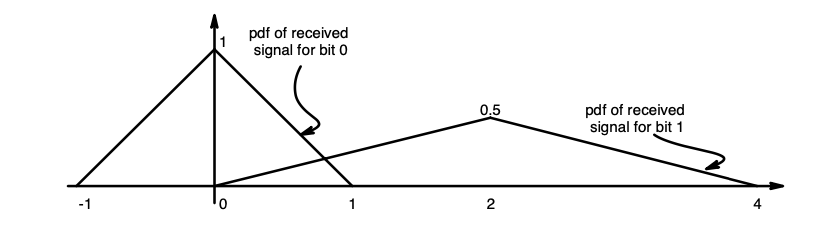
\includegraphics[width=0.5\columnwidth]{figs/fig_20.png}
    \caption{for q-48 and 49}
    \label{fig:placeholder_20}
\end{figure}
 
\item If the detection threshold is 1, the BER will be
\begin{multicols}{4}
\begin{enumerate}
\item $\frac{1}{2}$
\item $\frac{1}{4}$
\item $\frac{1}{8}$
\item $\frac{1}{16}$
\end{enumerate}
\end{multicols}
\hfill \brak{\text{GATE EC 2013}}

\item The optimum threshold to achieve minimum bit error rate \brak{BER} is
\begin{multicols}{4}
\begin{enumerate}
\item $\frac{1}{2}$
\item $\frac{4}{5}$
\item 1
\item $\frac{3}{2}$
\end{enumerate}
\end{multicols}
\hfill \brak{\text{GATE EC 2013}}

Common data for q-50 and q-51 

Consider the following $\figref{fig:placeholder_21}$. 
\begin{figure}[H]
    \centering
    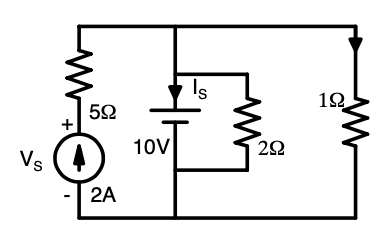
\includegraphics[width=0.5\columnwidth]{figs/fig_21.png}
    \caption{for q-50 and 51}
    \label{fig:placeholder_21}
\end{figure}

\item The current $I_s$ in Amps in the voltage source, and voltage $V_s$ in Volts across the current source respectively, are
\begin{multicols}{4}
\begin{enumerate}
\item $13, -20$
\item $8, -10$
\item $-8, 20$
\item $-13, 20$
\end{enumerate}
\end{multicols}
\hfill \brak{\text{GATE EC 2013}}



\item The current in the $1 \ohm$ resistor in Amps is
\begin{multicols}{4}
\begin{enumerate}
\item $2$
\item $3.33$
\item $10$
\item $12$
\end{enumerate}
\end{multicols}
\hfill \brak{\text{GATE EC 2013}}

Common data for q52 and q53

A monochromatic plane wave of wavelength $\lambda = 600\mu m$ is propagating in the direction as shown in the $\figref{fig:placeholder_22}$ below. $\vec{E_i}$ , $\vec{E_r}$ , and $\vec{E_t}$ denote incident, reflected, and transmitted electric field vectors associated with the wave.
\begin{figure}[H]
    \centering
    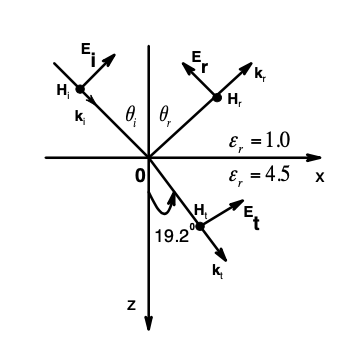
\includegraphics[width=0.5\columnwidth]{figs/fig_22.png}
    \caption{for q-52 and 53}
    \label{fig:placeholder_22}
\end{figure}

\item The angle of incidence $\theta_i$ and the expression for $\vec{E_i}$ is 
\begin{enumerate}
    \item $60^{\circ}$ and $\frac{E_o}{\sqrt{2}} \brak{\hat{a_x} - \hat{a_z}} e^{-j\frac{\pi \times 10^4 \brak{x+z} }{3\sqrt{2}}} V/m$
    \item $45^{\circ}$ and $\frac{E_o}{\sqrt{2}} \brak{\hat{a_x} + \hat{a_z}} e^{-j\frac{\pi \times 10^4 z }{3\sqrt{2}}} V/m$
    \item $45^{\circ}$ and $\frac{E_o}{\sqrt{2}} \brak{\hat{a_x} - \hat{a_z}} e^{-j\frac{\pi \times 10^4 \brak{x+z} }{3\sqrt{2}}} V/m$
    \item $60^{\circ}$ and $\frac{E_o}{\sqrt{2}} \brak{\hat{a_x} + \hat{a_z}} e^{-j\frac{\pi \times 10^4 z }{3\sqrt{2}}} V/m$
\end{enumerate}

\item The expression for $\vec{E_r}$ is
\begin{enumerate}
    \item $0.23 \frac{E_o}{\sqrt{2}}  \brak{ \hat{a_x} + \hat{a_z}} e^{-j\frac{\pi \times 10^4 \brak{x-z} }{3\sqrt{2}}}$
    \item $- \frac{E_o}{\sqrt{2}}  \brak{ \hat{a_x} + \hat{a_z}} e^{-j\frac{\pi \times 10^4 z }{3\sqrt{2}}}$
    \item $0.44 \frac{E_o}{\sqrt{2}}  \brak{ \hat{a_x} + \hat{a_z}} e^{-j\frac{\pi \times 10^4 \brak{x-z} }{3\sqrt{2}}}$
    \item $ \frac{E_o}{\sqrt{2}}  \brak{ \hat{a_x} + \hat{a_z}} e^{-j\frac{\pi \times 10^4 \brak{x+z} }{3\sqrt{2}}}$
\end{enumerate}

Common Data for q-54 and q-55

The state diagram of a system is shown below in $\figref{fig:placeholder_23}$. A system is described by the state-variable equations
\begin{align*}
    \dot{X} = AX + Bu; \ \ \ \ y= CX+Du
\end{align*}
\begin{figure}[H]
    \centering
    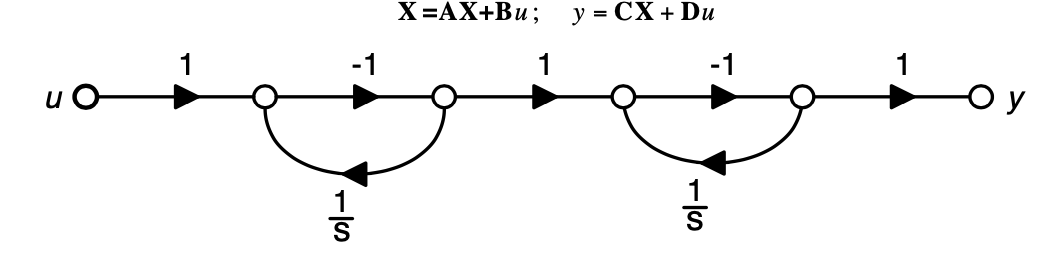
\includegraphics[width=0.5\columnwidth]{figs/fig_23.png}
    \caption{for q-54 and 55}
    \label{fig:placeholder_23}
\end{figure}
\item The state-variable equations of the system shown in the figure above are
\begin{multicols}{2}
\begin{enumerate}
    \item $\dot{X}= \myvec{-1&&0\\1&&-1} X + \myvec{-1 \\ 1} u$ \\ y=\myvec{1 && -1}X + u
    \item $\dot{X}= \myvec{-1&&0\\-1&&-1} X + \myvec{-1 \\ 1} u$ \\ y=\myvec{-1 && -1}X + u
    \item $\dot{X}= \myvec{-1&&0\\-1&&-1} X + \myvec{-1 \\ 1} u$ \\ y=\myvec{-1 && -1}X - u
    \item $\dot{X}= \myvec{-1&&-1\\0&&-1} X + \myvec{-1 \\ 1} u$ \\ y=\myvec{1 && -1}X - u
\end{enumerate}
\end{multicols}

\item The state transition matrix $e^{At}$ of the system shown in the figure above is
\begin{multicols}{4}
    \begin{enumerate}
        \item $\myvec{e^{-t} && 0 \\ te^{-t} && e^{-t}}$
        \item $\myvec{e^{-t} && 0 \\ -te^{-t} && e^{-t}}$
        \item $\myvec{e^{-t} && 0 \\ e^{-t} && e^{-t}}$
        \item $\myvec{e^{-t} && -te^{-t} \\ 0 && e^{-t}}$
    \end{enumerate}
\end{multicols}

\item Choose the grammatically CORRECT sentence:
\begin{enumerate}
\item Two and two add four.
\item Two and two become four.
\item Two and two are four.
\item Two and two make four.
\end{enumerate}
\hfill \brak{\text{GATE EC 2013}}

\item Statement: You can always give me a ring whenever you need.  
Which one of the following is the best inference from the above statement?
\begin{enumerate}
\item Because I have a nice caller tune.
\item Because I have a better telephone facility.
\item Because a friend in need is a friend indeed.
\item Because you need not pay towards the telephone bills when you give me a ring.
\end{enumerate}
\hfill \brak{\text{GATE EC 2013}}

\item In the summer of $2012$, in New Delhi, the mean temperature of Monday to Wednesday was $41^\circ\text{C}$ and of Tuesday to Thursday was $43^{\circ}\text{C}$. If the temperature on Thursday was $15 \%$ higher than that of Monday, then the temperature in $^\circ\text{C}$ on Thursday was
\begin{multicols}{4}
\begin{enumerate}
\item $40$
\item $43$
\item $46$
\item $49$
\end{enumerate}
\end{multicols}
\hfill \brak{\text{GATE EC 2013}}

\item Complete the sentence: Dare $\underline{\ \ \ } $ mistakes.
\begin{multicols}{4}
\begin{enumerate}
\item commit
\item to commit
\item committed
\item committing
\end{enumerate}
\end{multicols}
\hfill \brak{\text{GATE EC 2013}}

\item They were requested not to \textbf{quarrel} with others.  
Which one of the following options is the closest in meaning to the word quarrel?
\begin{multicols}{4}
\begin{enumerate}
\item make out
\item call out
\item dig out
\item fall out
\end{enumerate}
\end{multicols}
\hfill \brak{\text{GATE EC 2013}}

\item A car travels $8$ km in the first quarter of an hour, $6$ km in the second quarter and $16$ km in the third quarter. The average speed of the car in km per hour over the entire journey is
\begin{multicols}{4}
\begin{enumerate}
\item 30
\item 36
\item 40
\item 24
\end{enumerate}
\end{multicols}
\hfill \brak{\text{GATE EC 2013}}

\item Find the sum to \(n\) terms of the series \(10 + 84 + 734 + \ldots\)
\begin{multicols}{2}
\begin{enumerate}
\item $\frac{9\brak{9^n - 1}}{10 + 1}$
\item $\frac{9\brak{9^n - 1}}{8 + n}$
\item $\frac{9\brak{9^n - 1}}{8 + n^2}$
\item $\frac{9\brak{9^n - 1}}{8} + n^2$
\end{enumerate}
\end{multicols}
\hfill \brak{\text{GATE EC 2013}}

\item \textbf{Statement:} There were different streams of freedom movements in colonial India carried out by the moderates, liberals, radicals, socialists, and so on.  
Which one of the following is the best inference from the above statement?

\begin{enumerate}
\item The emergence of nationalism in colonial India led to our Independence.
\item Nationalism in India emerged in the context of colonialism.
\item Nationalism in India is homogeneous.
\item Nationalism in India is heterogeneous.
\end{enumerate}
\hfill \brak{\text{GATE EC 2013}}

\item The set of values of $p$ for which the roots of the equation $3x^2 + 2x + p\brak{p - 1} = 0$ are of opposite sign is
\begin{multicols}{4}
\begin{enumerate}
\item $\brak{-\infty, 0}$
\item $\brak{0, 1}$
\item $\brak{1, \infty}$
\item $\brak{0,\infty}$
\end{enumerate}
\end{multicols}
\hfill \brak{\text{GATE EC 2013}}

\item What is the chance that a leap year, selected at random, will contain $53$ Saturdays?
\begin{multicols}{4}
\begin{enumerate}
\item $\frac{2}{7}$
\item $\frac{3}{7}$
\item $\frac{1}{7}$
\item $\frac{5}{7}$
\end{enumerate}
\end{multicols}
\hfill \brak{\text{GATE EC 2013}}















\end{enumerate}


\end{document}
